% -------------------------------------------------------

%   LaTeX日常文件模板 by Meng Zhiran

%   demo.tex : 与普通的main.tex一致,可以在编译自己的文档时旁边开一个demo,方便copy代码

% -------------------------------------------------------

\documentclass[a4paper,12pt]{article}

% -------------------------------------------------------

%   LaTeX日常文件模板 by Meng Zhiran

%   packages.tex : 宏包引用文件,请在不会引起宏包冲突的前提下增加或删除宏包

% -------------------------------------------------------

% -----------------宏包功能简介与使用手册------------------

% (1){geometry}包:       设置页面的左、右、上、下页边距 [https://texdoc.org/serve/geometry/0]
% (2){fancyhdr}包:       提供页眉页脚设置 [https://texdoc.org/serve/fancyhdr/0]
% (3){indentfirst}包:    控制段落的首行缩进 [https://texdoc.org/serve/indenfirst/0]
% (4){setspace}包:       控制行间距(非段落间距,段落间距由documentclass控制) [https://texdoc.org/serve/setspace/0]
% (5){fontspec}包:       自定义文档字体大小与样式,英文模板中不含此包,会报错 [https://texdoc.org/serve/fontspec/0]
% (6){tocloft}包:        控制目录格式,提供插图目录和表格目录 [https://texdoc.org/serve/tocloft/0]
% (7){chngcntr}包:       计数器,允许图、表等分章节重新编号 [https://texdoc.org/serve/chngcntr/0]   
% (8){lastpage}包:       允许调用页码 [https://texdoc.org/serve/lastpage/0]
% (9){amssymb}包:        提供LaTeX数学符号排版环境 [https://texdoc.org/serve/amssymb/0]
% (10){amsmath}包:       提供LaTeX数学公式排版环境 [https://texdoc.org/serve/amsmath/0]
% (11){xcolor}包:        为文档添加颜色 [https://texdoc.org/serve/xcolor/0]
% (12){colortbl}包:      为表格添加颜色 [https://texdoc.org/serve/colortbl/0]
% (13){diagbox}包:       制作斜线表头 [https://texdoc.org/serve/diagbox/0]
% (14){longtable}包:     制作可跨页的长表格 [https://texdoc.org/serve/longtable/0]
% (15){multirow}包:      控制合并单元格操作 [https://texdoc.org/serve/multirow/0]
% (16){makecell}包:      控制单元格换行,避免长文本溢出 [https://texdoc.org/serve/makecell/0]
% (17){booktabs}包:      用于绘制三线表 [https://texdoc.org/serve/booktabs/0]
% (18){rotating}包:      用于旋转表格 [https://texdoc.org/serve/rotating/0]
% (19){graphicx}包:      提供LaTeX插图环境 [https://texdoc.org/serve/graphicx/0]
% (20){float}包:         提供浮动体环境 [https://texdoc.org/serve/float/0]
% (21){caption}包:       允许设置图表标题 [https://texdoc.org/serve/caption/0]
% (22){subfig}包:        允许插入多张子图 [https://texdoc.org/serve/subfig/0]
% (23){chemformula}包:   快速输入化学方程式 [https://texdoc.org/serve/chemformula/0]   
% (24){chemfig}包:       快速输入化学结构式 [https://texdoc.org/serve/chemfig/0]
% (25){hyperref}包:      控制超链接格式 [https://texdoc.org/serve/hyperref/0]
% (26){listings}包:      允许排版各种编程语言的源代码 [https://texdoc.org/serve/listings/0]
% (27){algorithm2e}包:   允许排版算法和伪代码 [https://texdoc.org/serve/algorithm2e/0]
% (28){enumerate}包:     允许使用不同类型的有序列表 [https://texdoc.org/serve/enumerate/0]
% (29){enumitem}包:      允许自定义列表格式 [https://texdoc.org/serve/enumitem/0]
% (30){pdfpages}包:      允许在文档中插入PDF页面 [https://texdoc.org/serve/pdfpages/0]
% (31){natbib}包:        提供Nature期刊标准引用格式 [https://texdoc.org/serve/natbib/0]
% (32){lipsum}包:        生成随机文本,用于测试 [https://texdoc.org/serve/lipsum/0]
% (33){amsthm}包:        提供LaTeX数学定理环境 [https://texdoc.org/serve/amsthm/0]
% (34){amsfonts}包:      提供LaTeX数学字体 [https://texdoc.org/serve/amsfonts/0]
% -----------------宏包功能简介与使用手册------------------


% -----------------宏包引用------------------
\usepackage[left=1.5cm,right=1.5cm,top=2cm,bottom=1.5cm]{geometry}
\usepackage{fancyhdr}
\usepackage{indentfirst}
\usepackage{setspace}
\usepackage{fontspec}
\usepackage{tocloft}
\usepackage{chngcntr}
\usepackage{lastpage}
\usepackage{amssymb}
\usepackage{amsmath}
\usepackage{amsthm}
\usepackage{amsfonts}
\usepackage[table]{xcolor}
\usepackage{colortbl}
\usepackage{diagbox}
\usepackage{longtable}
\usepackage{makecell}
\usepackage{multirow}
\usepackage{booktabs}
\usepackage[figuresright]{rotating}
\usepackage{graphics}
\usepackage{float} 
\usepackage[font=small,labelfont=bf,labelsep=none]{caption}
\usepackage{subfig}
\usepackage{chemformula}
\usepackage{chemfig}
\usepackage[colorlinks,linkcolor=black]{hyperref}
\usepackage{listings}
\usepackage[ruled,vlined]{algorithm2e}
\usepackage{enumerate}
\usepackage{enumitem}
\usepackage{pdfpages}
\usepackage[compress]{natbib}
\usepackage{lipsum}

% -----------------宏包引用------------------


% -------------------------------------------------------

%   LaTeX日常文件模板 by Meng Zhiran

%   introductory.tex : 导言区设置文件,设置编号规则、引用上标、页眉页脚、超链接等

% -------------------------------------------------------

% 目录设置为居中
\renewcommand{\cfttoctitlefont}{\hfill\Large\bfseries}
\renewcommand{\cftaftertoctitle}{\hfill}

\captionsetup{labelsep=quad}% 设置图表标题与编号之间的距离

\counterwithin{figure}{section} % 让图编号分章节编号
\counterwithin{table}{section}  % 让表编号分章节编号
\numberwithin{equation}{section}% 让公式编号分章节编号

\makeatletter
\newcommand\dlmu[2][5cm]{\hskip1pt\underline{\hb@xt@ #1{\hss#2\hss}}\hskip3pt} % 使用自定义的\dlmu命令创造指定长度的下划线,默认5cm
\makeatother

\newcommand{\Emph}[1]{\textbf{\emph{#1}}}% 使用自定义的\Emph命令创造加粗斜体字

\hypersetup{hidelinks} %使超链接文本与周围文本无视觉差异

% \setlength{\abovecaptionskip}{0pt} %调整标题与图距离

% 页眉页脚设置
\pagestyle{fancy}

\fancyhf{}
\fancyhead[L]
	{
		\hspace{0cm}
		\begin{minipage}[b]{0.05\linewidth}
			
\includegraphics[height=8mm]{Graph/sjtu_sign_en.png}
		\end{minipage}
	}

\fancyhead[R]{\footnotesize{A Test fancyhead}}
\fancyfoot[C]{\thepage}

% 设置代码高亮颜色
\definecolor{dkgreen}{rgb}{0,0.6,0}
\definecolor{mauve}{rgb}{0.58,0,0.82}

% Python的代码风格设置
\lstdefinestyle{Python}{
  language=Python,
  basicstyle=\ttfamily\small,
  keywordstyle=\color{blue},
  commentstyle=\color{dkgreen},
  stringstyle=\color{mauve},
  breaklines=true,
  breakatwhitespace=true,
  numbers=left,
  numberstyle=\tiny\color{gray},
  numbersep=10pt,
  tabsize=3,
  frame=single
}

% R的代码风格设置
\lstdefinestyle{R}{
  language=R,
  basicstyle=\ttfamily\small,
  keywordstyle=\color{red},
  commentstyle=\color{olive},
  stringstyle=\color{purple},
  breaklines=true,
  breakatwhitespace=true,
  numbers=left,
  numberstyle=\tiny\color{gray},
  numbersep=10pt,
  tabsize=3,
  frame=single
}

% 将Reference居中
\def\bibsection{\centering\section*{\refname}}

\title{\textbf{\LaTeX Demo}}

\author{Meng Zhiran}

\date{\today}

\begin{document}

\tableofcontents

\thispagestyle{empty}
\newpage

\listoffigures
\listoftables
\listofalgorithms
\thispagestyle{empty}
\newpage

\maketitle

\setcounter{page}{1}
\thispagestyle{fancy}


\section{TEXT}

According to the study conducted by Smith and colleagues \cite{bhagat2017,bittencourt2022,brennan2017,doblhofer2015}, the use of artificial intelligence in software development
has significantly increased productivity. The study found that AI-powered programming assistants, such as GitHub Copilot, can help 
developers write code more efficiently by suggesting code completions and detecting bugs early in the development process.

\begin{itemize}
    \item ABCDEFG
    \item \emph{HIJKLMN}
    \item \textbf{OPQRSTU}
    \item \Emph{VWXYZ}
\end{itemize}

\lipsum[1]

% enumerate可选参数:[1]表示编号从1开始,[a]表示小写字母编号,[A]表示大写字母编号,[i]表示小写罗马数字编号,[I]表示大写罗马数字编号

\begin{enumerate}
    \item ABCDEFG
    \item \emph{HIJKLMN}
    \item \textbf{OPQRSTU}
    \item \Emph{VWXYZ}
\end{enumerate}

\lipsum[1]

\begin{description}
    \item[Description1] ABCDEFG
    \item[\emph{Description2}] \emph{HIJKLMN}
\end{description}


\section{FIGURES}

\subsection{Single Figure}

\lipsum[1]

\begin{figure}[htbp]
    \centering
    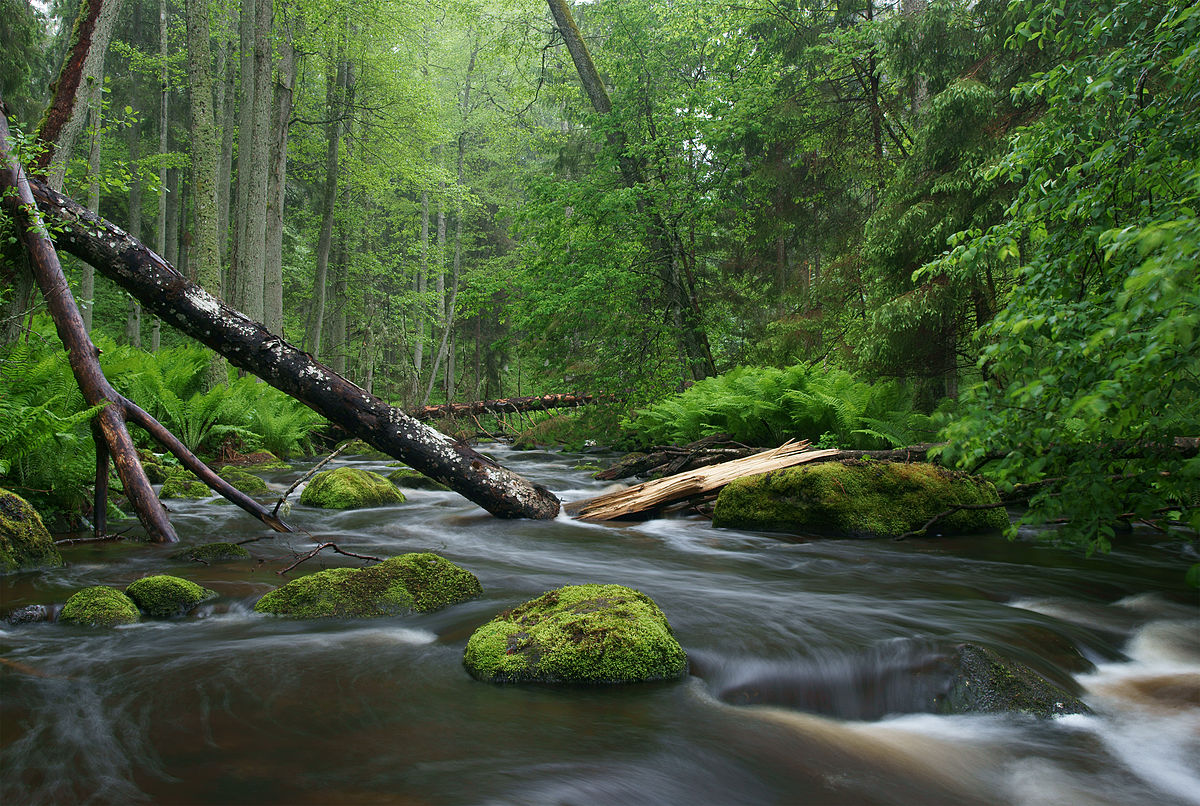
\includegraphics[width=0.6\textwidth]{Graph/test}
    \caption{Test Figure 1}
    \label{fig1}
\end{figure}


\subsection{Subfigures}

\lipsum[1]

\begin{figure}[htbp]
    \centering
    \subfloat[Subfigure 1]{
\includegraphics[width=0.35\textwidth]{Graph/test1}\label{fig:sub1}}
    \hspace{0.05\textwidth} % Adjust this value to control the gap
    \subfloat[Subfigure 2]{
\includegraphics[width=0.35\textwidth]{Graph/test1}\label{fig:sub2}}
    \\
    \subfloat[Subfigure 3]{
\includegraphics[width=0.35\textwidth]{Graph/test1}\label{fig:sub3}}
    \hspace{0.05\textwidth} % Adjust this value to control the gap
    \subfloat[Subfigure 4]{
\includegraphics[width=0.35\textwidth]{Graph/test1}\label{fig:sub4}}
    \caption{Caption for the whole figure}
    \label{fig:whole2}
\end{figure}

\subsection{Complex figure}

\lipsum[1]

\begin{figure}[htbp]
    \centering
    \subfloat[Subfigure 1]{
\includegraphics[width=0.35\textwidth]{Graph/test1}\label{fig:subsub1}}
    \hspace{0.05\textwidth} % Adjust this value to control the gap
    \subfloat[Subfigure 2]{
\includegraphics[width=0.35\textwidth]{Graph/test1}\label{fig:subsub2}}
    \\
    \subfloat[Subfigure 3]{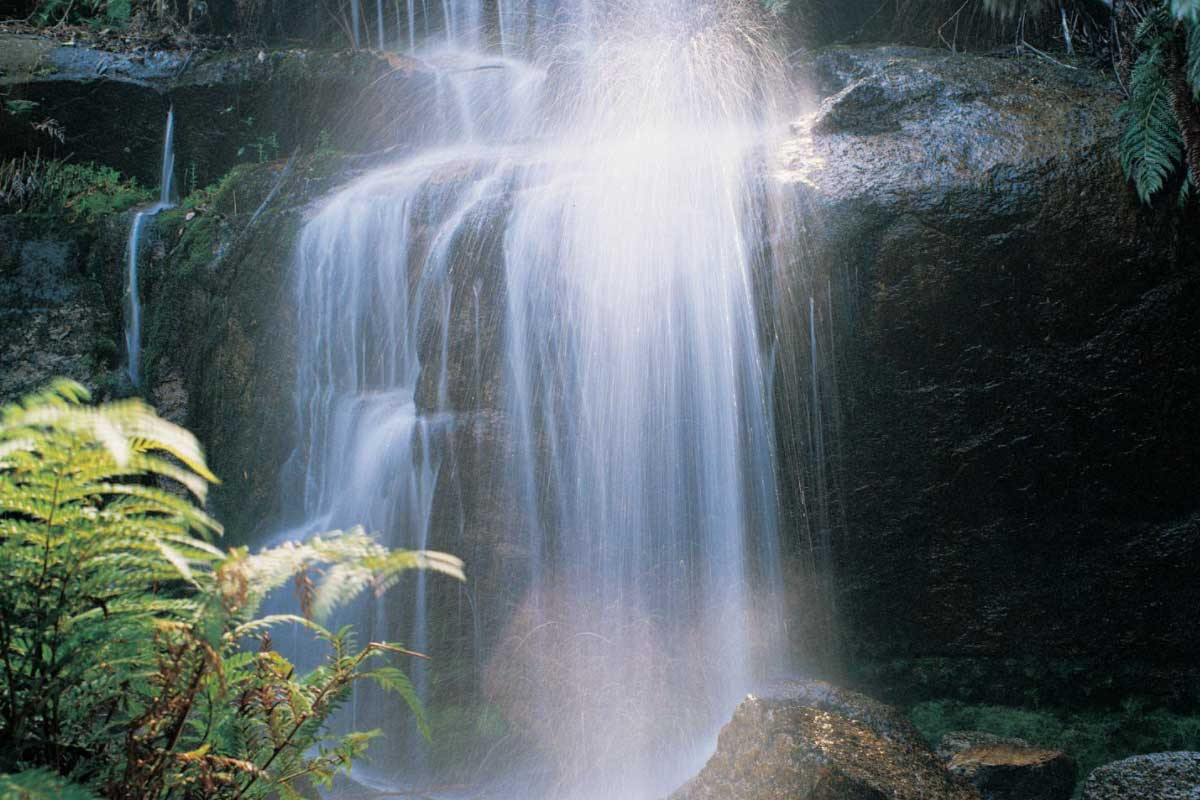
\includegraphics[width=0.35\textwidth]{Graph/test3}\label{fig:subsub3}}
    \hspace{0.05\textwidth} % Adjust this value to control the gap
    \subfloat[Subfigure 4]{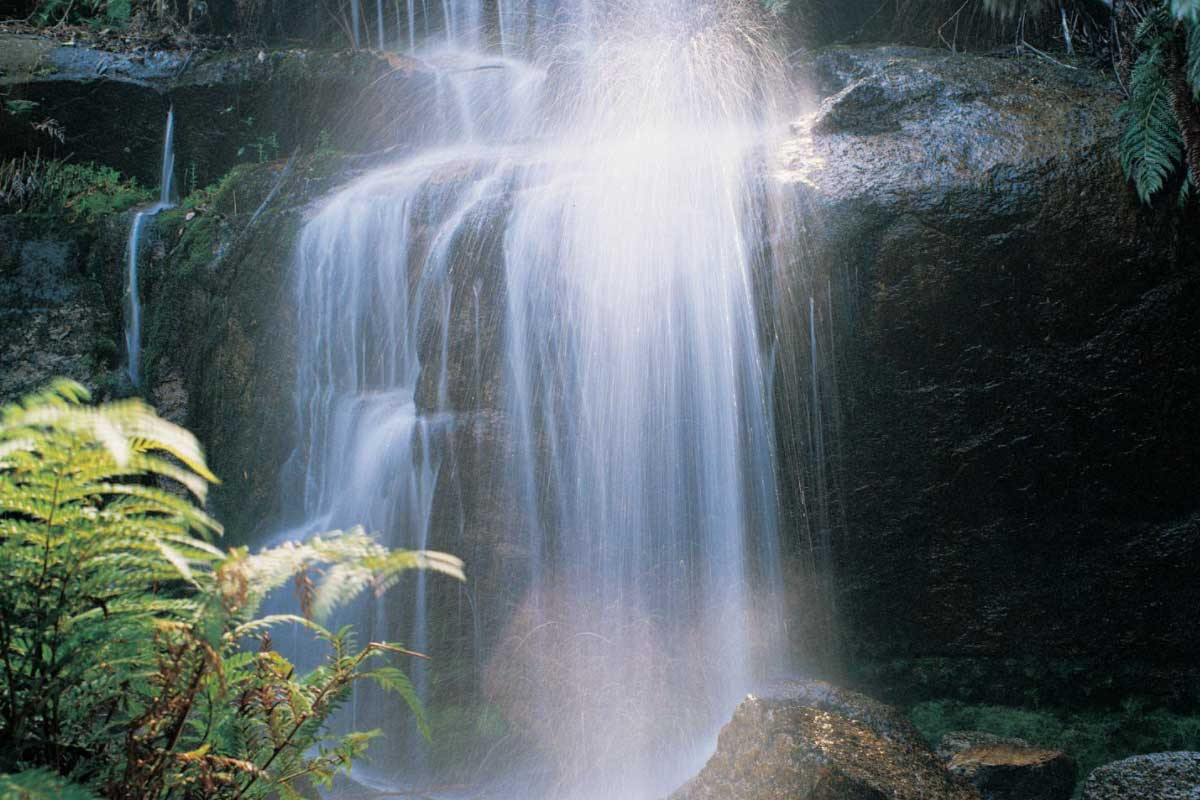
\includegraphics[width=0.35\textwidth]{Graph/test3}\label{fig:subsub4}}
    \\
    \subfloat[Subfigure 5]{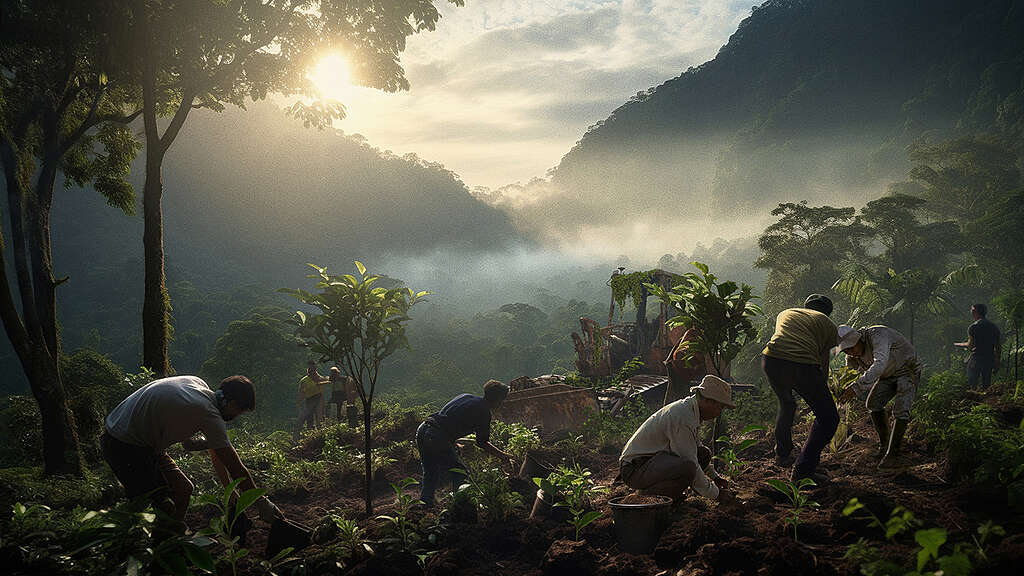
\includegraphics[width=0.75\textwidth]{Graph/test2}\label{fig:subsub5}}
    \caption{Caption for the complex figure}
    \label{fig:whole3}
\end{figure}


\section{TABLES}

\subsection{Small Table}

\lipsum[1]

\begin{table}[htbp]
    \centering
    \caption{Caption for the table}
    \begin{tabular}{ccc}
        \toprule
        Header 1 & Header 2 & Header 3 \\
        \midrule
        Cell 1 & Cell 2 & Cell 3 \\
        Cell 4 & Cell 5 & Cell 6 \\
        \bottomrule
    \end{tabular}
    \label{tab:mytable}
\end{table}

\subsection{Large Rotated Table}

\lipsum[1]

\begin{sidewaystable}
    \centering
    \caption{Caption for the large table}
    \begin{tabular}{cccccccccc}
        \toprule
        Header 1 & Header 2 & Header 3 & Header 4 & Header 5 & Header 6 & Header 7 & Header 8 & Header 9 & Header 10 \\
        \midrule
        Cell 1 & Cell 2 & Cell 3 & Cell 4 & Cell 5 & Cell 6 & Cell 7 & Cell 8 & Cell 9 & Cell 10 \\ [5ex]
        Cell 11 & Cell 12 & Cell 13 & Cell 14 & Cell 15 & Cell 16 & Cell 17 & Cell 18 & Cell 19 & Cell 20 \\ [5ex]
        Cell 21 & Cell 22 & Cell 23 & Cell 24 & Cell 25 & Cell 26 & Cell 27 & Cell 28 & Cell 29 & Cell 30 \\ [5ex]
        Cell 31 & Cell 32 & Cell 33 & Cell 34 & Cell 35 & Cell 36 & Cell 37 & Cell 38 & Cell 39 & Cell 40 \\ [5ex]
        Cell 41 & Cell 42 & Cell 43 & Cell 44 & Cell 45 & Cell 46 & Cell 47 & Cell 48 & Cell 49 & Cell 50 \\ [5ex]
        Cell 51 & Cell 52 & Cell 53 & Cell 54 & Cell 55 & Cell 56 & Cell 57 & Cell 58 & Cell 59 & Cell 60 \\ [5ex]
        Cell 61 & Cell 62 & Cell 63 & Cell 64 & Cell 65 & Cell 66 & Cell 67 & Cell 68 & Cell 69 & Cell 70 \\ [5ex]
        Cell 71 & Cell 72 & Cell 73 & Cell 74 & Cell 75 & Cell 76 & Cell 77 & Cell 78 & Cell 79 & Cell 80 \\ [5ex]
        Cell 81 & Cell 82 & Cell 83 & Cell 84 & Cell 85 & Cell 86 & Cell 87 & Cell 88 & Cell 89 & Cell 90 \\ [5ex]
        Cell 91 & Cell 92 & Cell 93 & Cell 94 & Cell 95 & Cell 96 & Cell 97 & Cell 98 & Cell 99 & Cell 100 \\

        \bottomrule
    \end{tabular}
    \label{tab:myLargeTable}
\end{sidewaystable}


\section{FORMULAS}

\subsection{Inline Mathmetical Expression}

We compared the number of colonies in the control ($n=3$) and experimental ($n=3$) groups

\subsection{Formula Environment}

\lipsum[1]

$$
    \overbrace{1+2+\cdots+100}
$$

\lipsum[1]

\begin{equation}
    \frac{k}{k-1} = 0.5
\end{equation}

    
\subsection{Large Formula}

\lipsum[1]

$$
    \begin{aligned}
        \nabla \cdot \mathbf{E} &= \frac {\rho} {\varepsilon_0} \\
        \nabla \cdot \mathbf{B} &= 0 \\
        \nabla \times \mathbf{E} &= -\frac{\partial \mathbf{B}} {\partial t} \\
        \nabla \times \mathbf{B} &= \mu_0\mathbf{J} + \mu_0\varepsilon_0\frac{\partial \mathbf{E}} {\partial t}
    \end{aligned}
$$

\lipsum[1]

\begin{equation}
    \begin{cases}
        3x + 5y + z &= 1 \\
        7x - 2y + 4z &= 2 \\
        -6x + 3y + 2z &= 3
    \end{cases}
\end{equation}


\subsection{Theory}

\lipsum[1]

\newtheorem{theory}{Theory}

\begin{theory}
    Here is the statement of your theory.
\end{theory}

\lipsum[2]

\section{CODES}

\subsection{Algorithm}

\lipsum[3]

\begin{algorithm}
    \DontPrintSemicolon
    \KwData{$G=(X,U)$ such that $G^{tc}$ is an order.}
    \KwResult{$G'=(X,V)$ with $V\subseteq U$ such that $G'^{tc}$ is an
    interval order.}
    \Begin{
    $V \longleftarrow U$\;
    $S \longleftarrow \emptyset$\;
    \For{$x\in X$}{
    $NbSuccInS(x) \longleftarrow 0$\;
    $NbPredInMin(x) \longleftarrow 0$\;
    $NbPredNotInMin(x) \longleftarrow |ImPred(x)|$\;
    }
    \For{$x \in X$}{
    \If{$NbPredInMin(x) = 0$ {\bf and} $NbPredNotInMin(x) = 0$}{
    $AppendToMin(x)$}
    }
    \nl\While{$S \neq \emptyset$}{\label{InRes1}
    \nlset{REM} remove $x$ from the list of $T$ of maximal index\;\label{InResR}
    \lnl{InRes2}\While{$|S \cap ImSucc(x)| \neq |S|$}{
    \For{$ y \in S-ImSucc(x)$}{
    \{ remove from $V$ all the arcs $zy$ : \}\;
    \For{$z \in ImPred(y) \cap Min$}{
    remove the arc $zy$ from $V$\;
    $NbSuccInS(z) \longleftarrow NbSuccInS(z) - 1$\;
    move $z$ in $T$ to the list preceding its present list\;
    \{i.e. If $z \in T[k]$, move $z$ from $T[k]$ to
    $T[k-1]$\}\;
    }
    $NbPredInMin(y) \longleftarrow 0$\;
    $NbPredNotInMin(y) \longleftarrow 0$\;
    $S \longleftarrow S - \{y\}$\;
    $AppendToMin(y)$\;
    }
    }
    $RemoveFromMin(x)$\;
    }
    }
    \caption{IntervalRestriction\label{IR}}
\end{algorithm}

\lipsum[2]

\subsection{Python Code}

\lipsum[1]


\begin{lstlisting}[style=Python]
    class Person:
    def __init__(self, name, age):
        self.name = name
        self.age = age

    def greet(self):
        print("Hello, my name is " + self.name + " and I am " + str(self.age) + " years old.")

class Student(Person):
    def __init__(self, name, age, grade):
        super().__init__(name, age)
        self.grade = grade

    def study(self):
        print(self.name + " is studying.")

alice = Student('Alice', 20, 'Sophomore')
alice.greet()
alice.study()

\end{lstlisting}

\subsection{R Code}

\lipsum[1]

\begin{lstlisting}[style=R]
    # Define a function to calculate the mean
    calculate_mean <- function(x) {
      sum_x <- sum(x)
      n <- length(x)
      mean_x <- sum_x / n
      return(mean_x)
    }
    
    # Define a function to calculate the variance
    calculate_variance <- function(x) {
      mean_x <- calculate_mean(x)
      squared_diffs <- (x - mean_x)^2
      sum_squared_diffs <- sum(squared_diffs)
      n <- length(x)
      variance_x <- sum_squared_diffs / (n - 1)
      return(variance_x)
    }
    
    # Use the functions
    x <- c(1, 2, 3, 4, 5)
    mean_x <- calculate_mean(x)
    variance_x <- calculate_variance(x)
    
    print(paste("Mean of x:", mean_x))
    print(paste("Variance of x:", variance_x))
\end{lstlisting}


\newpage

\bibliographystyle{unsrt}

\bibliography{ref.bib}

\end{document}